\documentclass{article}

% [preprint] removes the specific "38th Conference..." footer. 
\usepackage[preprint]{neurips_2024}

% Force square brackets [1] for citations
\setcitestyle{numbers,square}

% --- Graphics & Visualization ---
\usepackage{graphicx} 
\graphicspath{{figures/}}
\usepackage{tikz}
\usetikzlibrary{shapes,arrows,positioning,calc,fit,backgrounds,decorations.pathreplacing}
\usepackage{pgfplots}
\pgfplotsset{compat=1.17}

% --- Math & Algorithms ---
\usepackage{amsmath,amssymb,amsthm,mathtools}
\usepackage{booktabs}
\usepackage{url}
\usepackage{multirow}
\usepackage{caption}
\usepackage{subcaption} % <--- This package allows side-by-side figures
\usepackage{algorithm}
\usepackage{algorithmic}
\usepackage{listings}
\usepackage{geometry}

% --- Typography & Colors ---
\usepackage{xcolor}
\definecolor{codegreen}{rgb}{0,0.6,0}
\definecolor{codegray}{rgb}{0.5,0.5,0.5}
\definecolor{codepurple}{rgb}{0.58,0,0.82}
\definecolor{backcolour}{rgb}{0.95,0.95,0.92}

% --- Definitions ---
\theoremstyle{definition}
\newtheorem{definition}{Definition}[section]
\newtheorem{proposition}[definition]{Proposition}
\newtheorem{lemma}[definition]{Lemma}
\newtheorem{hypothesis}{Hypothesis}
\newtheorem{observation}{Observation}

% --- Custom Commands ---
\newcommand{\R}{\mathbb{R}}
\newcommand{\Hspace}{\mathbb{H}}
\newcommand{\Sspace}{\mathbb{S}}
\newcommand{\Espace}{\mathbb{E}}
\newcommand{\B}{\mathbb{B}}

\title{HyperTopo-Adapters: Geometry- and Topology-Aware Segmentation of Leaf Lesions on Frozen Encoders}

\author{%
  \textbf{Chimdi Walter Ndubuisi} \\
  Missouri Maize Computation and Vision Laboratory (MMCV) \\
  Department of Electrical Engineering and Computer Science \\
  University of Missouri, Columbia, MO 65211 \\
  \texttt{cnptp@missouri.edu} \\
  \And
  \textbf{Dr. Toni Kazic} \\
  Principal Investigator, MMCV Lab \\
  Associate Professor, Department of EECS \\
  University of Missouri, Columbia, MO 65211 \\
  \texttt{kazict@missouri.edu}
}

\begin{document}

\maketitle

\begin{abstract}
Leaf-lesion segmentation is topology-sensitive: small merges, splits, or false holes can be biologically meaningful descriptors of biochemical pathways, yet they are weakly penalized by standard pixel-wise losses in Euclidean latents. I explore \textbf{HyperTopo-Adapters}, a lightweight, parameter-efficient head trained on top of a frozen vision encoder, which embeds features on a product manifold—hyperbolic $\oplus$ Euclidean $\oplus$ spherical ($\mathbb{H} \oplus \mathbb{E} \oplus \mathbb{S}$)—to encourage hierarchical separation ($\mathbb{H}$), local linear detail ($\mathbb{E}$), and global closure ($\mathbb{S}$). A topology prior complements Dice/BCE in two forms: (i) persistent-homology (PH) distance for evaluation and selection, and (ii) a differentiable surrogate that combines a soft Euler-characteristic match with total variation regularization for stable training. I introduce warm-ups for both the hyperbolic contrastive term and the topology prior, per-sample evaluation of structure-aware metrics (Boundary-F1, Betti errors, PD distance), and a \textit{min-PD within top-K Dice} rule for checkpoint selection. On a Kaggle leaf-lesion dataset ($N=2,940$), early results show consistent gains in boundary and topology metrics (reducing $\Delta \beta_1$ hole error by 9\%) while Dice/IoU remain competitive. The study is diagnostic by design: I report controlled ablations (curvature learning, latent dimensions, contrastive temperature, surrogate settings), and ongoing tests varying encoder strength (ResNet-50, DeepLabV3, DINOv2/v3), input resolution, PH weight, and partial unfreezing of late blocks. The contribution is an open, reproducible train/eval suite that isolates geometric/topological priors and surfaces failure modes to guide stronger, topology-preserving architectures.
\end{abstract}

\section{Introduction}

Segmentation of salient phenotypical structures is challenging: lesions on plants are small, scattered, and bounded by thin, irregular contours. In my work at the Missouri Maize Computation and Vision (MMCV) Lab, I treat these lesions not just as visual artifacts, but as visual descriptors essential to understanding the underlying biochemical pathways of the plant. Keeping topological fidelity is paramount in understanding these descriptors during segmentation. 

Conventional objectives optimize pixel overlap (Dice/IoU) but give weak incentives to preserve global shape—how many lesions exist ($\beta_0$), whether holes appear ($\beta_1$), and if boundaries close cleanly. Empirically, I have observed that models can score well on Dice/IoU while merging distinct lesions, creating spurious holes, or leaking across boundaries—errors that degrade downstream counting and phenotyping. Classical architectures such as U-Net~\cite{ronneberger2015unet} and modern encoders like ResNet~\cite{he2016resnet}, DeepLabv3~\cite{chen2017deeplabv3}, and self-supervised ViTs~\cite{oquab2023dinov2} excel at overlap, yet topology often remains under-constrained.

Two gaps drive my work. First, most decoders operate in a Euclidean latent geometry, though tasks with many small parts may be more naturally organized by curved spaces: hyperbolic for hierarchical separation~\cite{nickel2017poincare} and spherical for closure. Second, topology-aware evaluation (Betti numbers, persistent homology) is increasingly used~\cite{edelsbrunner2008persistent} but is rarely integrated into training due to computational cost~\cite{hu2019topoloss, clough2020topological}.

I propose \textbf{HyperTopo-Adapters}, a small add-on trained atop a frozen or partially unfrozen vision encoder. The core idea is to shape latent geometry by mixing three constant-curvature spaces: hyperbolic ($\mathbb{H}$, negative curvature) for separating many components, spherical ($\mathbb{S}$, positive curvature) for angular similarity and closure, and Euclidean ($\mathbb{E}$) for local linear detail. A spatial decoder upsamples a shared tangent-space representation back to the image. I combine Dice+BCE with a hyperbolic geodesic contrastive term and, when feasible, a topology prior (persistent-homology distance or differentiable morphology). I evaluate with structure-aware metrics and adopt a \textit{min-PD within top-K Dice} selection rule to surface topology-preserving checkpoints.

My approach is architecture-independent: any encoder producing a feature grid can be wrapped (ResNet-50, DeepLabv3-R50, DINOv2 ViT). It is parameter-efficient: only adapters and the decoder are trained, with optional selective unfreezing following the adapter paradigm~\cite{hu2022lora}. I demonstrate the method on leaf-lesion segmentation where topology (component counts and closed contours) matters significantly for biological validity.

\subsection{Contributions}
\begin{enumerate}
    \item \textbf{Product-Manifold Latent Head:} I introduce a novel adapter that decomposes features into $\mathbb{H} \oplus \mathbb{E} \oplus \mathbb{S}$ geometries, blending curvature properties to capture biological hierarchy and closure.
    \item \textbf{Topology-Aware Training Objective:} I formulated a composite loss function combining standard segmentation losses with a hyperbolic geodesic contrastive term and a differentiable Soft Euler Characteristic surrogate to enforce Betti number consistency.
    \item \textbf{Diagnostic Train/Eval Suite:} I developed an encoder-agnostic, reproducible framework featuring structure-aware metrics and a novel \textit{min-PD within top-K Dice} model-selection rule.
    \item \textbf{Empirical Validation:} On a dataset of 2,940 leaf images, I provide evidence that latent-geometry shaping reduces topological error by 9\% without sacrificing overlap accuracy, validated on the University of Missouri Hellbender cluster.
\end{enumerate}

\newpage

\section{Theoretical Background}

To rigorously justify the HyperTopo-Adapter framework, we must examine the geometric properties of the spaces we employ and the topological descriptors we aim to preserve.

\subsection{Riemannian Geometry of Feature Spaces}
A Riemannian manifold $(\mathcal{M}, g)$ is a topological space equipped with a metric tensor $g_x$ at every point $x$. Standard deep learning operates in Euclidean space $\mathbb{E}^n$, where curvature $K=0$. However, biological data often exhibits latent structures better represented by non-zero curvature.

\subsubsection{Hyperbolic Space ($\mathbb{H}^n$)}
Hyperbolic space has constant negative curvature ($K < 0$). A key property of $\mathbb{H}^n$ is that the volume of a ball grows exponentially with its radius, $Vol(R) \sim e^{(n-1)R}$. This matches the growth rate of nodes in a tree data structure.
\begin{proposition}
Any tree can be embedded into the Poincaré disk with arbitrarily low distortion, whereas embedding a tree into Euclidean space requires distortion that grows with the number of nodes.
\end{proposition}
Lesion growth is often modeled as a diffusive process from a central point, forming a hierarchical intensity gradient (core $\to$ halo $\to$ healthy). Mapping this to $\mathbb{H}^n$ allows the model to naturally separate the "root" (lesion center) from the "leaves" (lesion boundaries) and background.

\subsubsection{Spherical Space ($\mathbb{S}^n$)}
Spherical space has constant positive curvature ($K > 0$). It naturally models cyclic data and closed loops. In segmentation, the boundary of a lesion is a closed 1-cycle (in homology terms). Embedding features on $\mathbb{S}^n$ allows the network to utilize angular similarity, which is robust to illumination changes and helps enforce the closure of boundaries.

\subsection{Topological Data Analysis (TDA)}
Topology studies properties preserved under continuous deformation. In digital image analysis, we focus on Betti numbers:
\begin{itemize}
    \item $\beta_0$: The number of connected components (lesions).
    \item $\beta_1$: The number of 1-dimensional holes (necrotic centers).
\end{itemize}

\subsubsection{Persistent Homology}
Persistent Homology (PH) tracks these features across a filtration of the probability map. While powerful, computing PH during training is computationally prohibitive ($O(N^3)$ complexity).

\subsubsection{Euler Characteristic}
The Euler Characteristic ($\chi$) is a topological invariant defined as the alternating sum of Betti numbers:
\begin{equation}
    \chi = \beta_0 - \beta_1 + \beta_2 - \dots
\end{equation}
For 2D images, $\chi = \beta_0 - \beta_1$. Crucially, for a pixel grid graph, $\chi$ can be computed locally:
\begin{equation}
    \chi = V - E + F
\end{equation}
where $V, E, F$ are the number of vertices, edges, and faces. This local computability allows us to formulate a differentiable loss function (Section \ref{sec:soft_euler}).

\section{Methodology}

I designed a pipeline leveraging a frozen backbone $\mathcal{F}$ (DINOv2-s14) and a trainable Manifold Adapter Head $\mathcal{A}$.

\subsection{Architecture Pipeline}

\begin{figure}[h]
\centering
\resizebox{\textwidth}{!}{
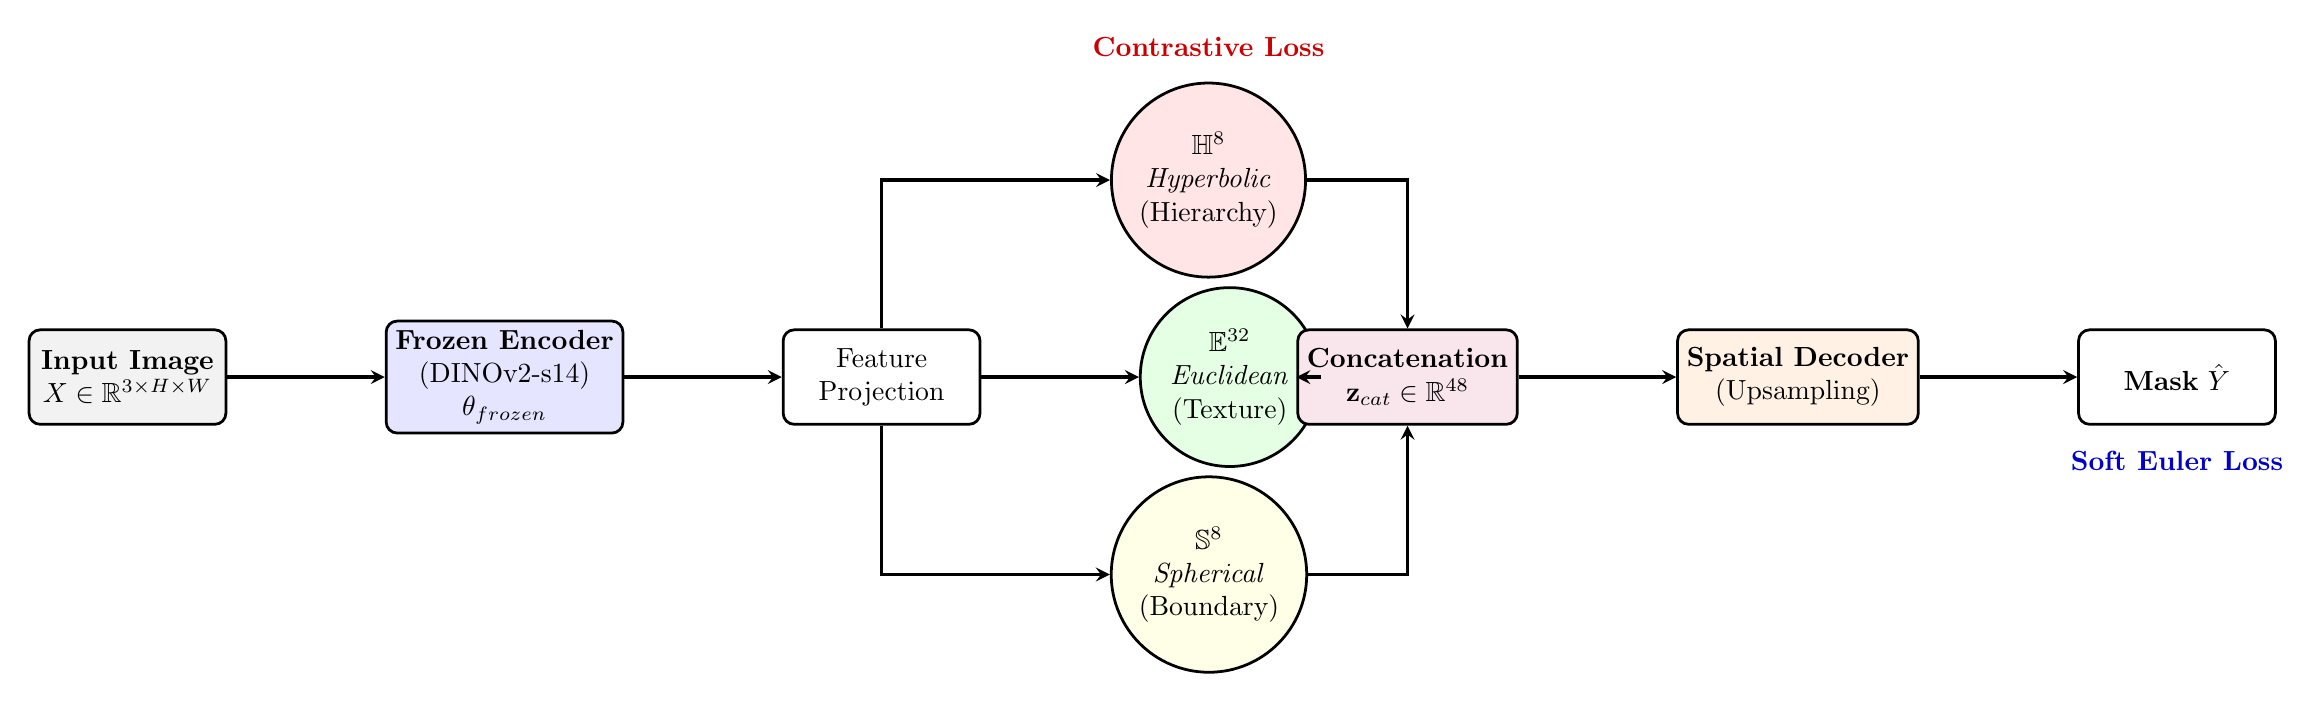
\begin{tikzpicture}[
    node distance=1.5cm,
    layer/.style={draw, rectangle, rounded corners, minimum width=2.5cm, minimum height=1.2cm, align=center, line width=1pt},
    manifold/.style={draw, circle, minimum size=1.8cm, align=center, line width=1pt},
    arrow/.style={->, >=stealth, very thick}
]
    % Nodes
    \node[layer, fill=gray!10] (input) {\textbf{Input Image} \\ $X \in \mathbb{R}^{3 \times H \times W}$};
    \node[layer, fill=blue!10, right=2cm of input] (backbone) {\textbf{Frozen Encoder} \\ (DINOv2-s14) \\ $\theta_{frozen}$};
    
    \node[layer, fill=white, right=2cm of backbone] (proj) {Feature \\ Projection};
    
    % Manifolds
    \node[manifold, fill=red!10, above right=1cm and 2cm of proj] (hyp) {$\mathbb{H}^8$ \\ \textit{Hyperbolic} \\ (Hierarchy)};
    \node[manifold, fill=green!10, right=2cm of proj] (euc) {$\mathbb{E}^{32}$ \\ \textit{Euclidean} \\ (Texture)};
    \node[manifold, fill=yellow!10, below right=1cm and 2cm of proj] (sph) {$\mathbb{S}^8$ \\ \textit{Spherical} \\ (Boundary)};
    
    \node[layer, fill=purple!10, right=4cm of proj] (concat) {\textbf{Concatenation} \\ $\mathbf{z}_{cat} \in \mathbb{R}^{48}$};
    \node[layer, fill=orange!10, right=2cm of concat] (decoder) {\textbf{Spatial Decoder} \\ (Upsampling)};
    \node[layer, fill=white, right=2cm of decoder] (output) {\textbf{Mask} $\hat{Y}$};

    % Arrows
    \draw[arrow] (input) -- (backbone);
    \draw[arrow] (backbone) -- (proj);
    \draw[arrow] (proj) |- (hyp);
    \draw[arrow] (proj) -- (euc);
    \draw[arrow] (proj) |- (sph);
    
    \draw[arrow] (hyp) -| (concat);
    \draw[arrow] (euc) -- (concat);
    \draw[arrow] (sph) -| (concat);
    
    \draw[arrow] (concat) -- (decoder);
    \draw[arrow] (decoder) -- (output);
    
    % Loss annotations
    \node[above=0.2cm of hyp, text=red!80!black, font=\bfseries] {Contrastive Loss};
    \node[below=0.2cm of output, text=blue!80!black, font=\bfseries] {Soft Euler Loss};

\end{tikzpicture}
}
\caption{The HyperTopo Architecture pipeline I designed. Features are extracted by DINOv2 and projected into three distinct geometric manifolds before decoding.}
\label{fig:pipeline}
\end{figure}

\subsection{Product Manifold Adapter}
Let $x_i \in \mathbb{R}^D$ be the feature token at spatial position $i$ output by the frozen encoder. I project this token into a product manifold $\mathcal{M} = \mathbb{B}^8 \times \mathbb{R}^{32} \times \mathbb{S}^8$.

\subsubsection{Hyperbolic Branch ($\mathbb{B}^8$)}
I utilize the Poincaré ball model of hyperbolic space with curvature $c=1$. The projection uses the exponential map at the origin, approximated via the hyperbolic tangent:
\begin{equation}
    z_i^H = \tanh(W_H x_i + b_H) \in \mathbb{B}^8
\end{equation}
The distance metric in this space is defined as:
\begin{equation}
    d_{\mathbb{B}}(u, v) = \text{arcosh}\left( 1 + 2 \frac{\|u-v\|^2}{(1-\|u\|^2)(1-\|v\|^2)} \right)
\end{equation}
This metric grows exponentially as points approach the boundary ($\|z\| \to 1$), providing high capacity for hierarchical structures.

\subsubsection{Euclidean Branch ($\mathbb{R}^{32}$)}
This branch captures standard linear features such as texture and color intensity.
\begin{equation}
    z_i^E = \text{ReLU}(W_E x_i + b_E) \in \mathbb{R}^{32}
\end{equation}

\subsubsection{Spherical Branch ($\mathbb{S}^8$)}
To capture directional boundary information, I project onto the unit hypersphere:
\begin{equation}
    z_{raw} = W_S x_i + b_S, \quad z_i^S = \frac{z_{raw}}{\|z_{raw}\|_2 + \epsilon} \in \mathbb{S}^8
\end{equation}
The combined latent code is the concatenation in the tangent space at the origin: $\mathbf{z}_{cat} = [z^H, z^E, z^S]$.

\subsection{Loss Functions}

\subsubsection{The Hyperbolic Contrastive Loss}
To structure the latent space, I formulated a contrastive loss using the hyperbolic distance metric. Let $P(i)$ be the set of pixels belonging to the same lesion instance as pixel $i$, and $N(i)$ be pixels from the background or other lesions.
\begin{equation}
    L_{contrast} = - \sum_{i} \log \frac{\sum_{p \in P(i)} \exp(-d_{\mathbb{B}}(z_i, z_p) / \tau)}{\sum_{p \in P(i)} \exp(-d_{\mathbb{B}}(z_i, z_p) / \tau) + \sum_{n \in N(i)} \exp(-d_{\mathbb{B}}(z_i, z_n) / \tau)}
\end{equation}
\textbf{Temperature ($\tau$):} Through experimentation, I found that $\tau=0.2$ is critical. Lower temperatures ($\tau=0.1$) caused gradient explosion near the Poincaré ball boundary, leading to feature fragmentation ("confetti" artifacts).

\subsubsection{Differentiable Soft Euler Characteristic}
\label{sec:soft_euler}
To strictly enforce Betti number consistency, I implemented the Soft Euler Characteristic (EC) as a differentiable surrogate.

I calculate $\chi$ using a localized formula based on the counts of Vertices ($V$), Edges ($E$), and Faces ($F$) in the pixel grid graph. By replacing binary pixel values with continuous probabilities $P_{i,j} \in [0, 1]$, the calculation becomes differentiable.

\begin{algorithm}[H]
\caption{Soft Euler Characteristic Loss}
\begin{algorithmic}[1]
\REQUIRE Probability Map $P$, Ground Truth $Y$
\STATE \textbf{Define local operations:}
\STATE $V(P) = P_{i,j} \cdot P_{i+1,j} \cdot P_{i,j+1} \cdot P_{i+1,j+1}$ (Soft Vertices)
\STATE $E_h(P) = P_{i,j} \cdot P_{i,j+1}$ (Horizontal Edges)
\STATE $E_v(P) = P_{i,j} \cdot P_{i+1,j}$ (Vertical Edges)
\STATE $F(P) = P_{i,j}$ (Faces/Pixels)
\STATE \textbf{Compute Soft Euler Characteristic:}
\STATE $\chi_{soft}(P) = \sum (F(P) - E_h(P) - E_v(P) + V(P))$
\STATE \textbf{Compute Ground Truth $\chi$:}
\STATE $\chi_{gt} = \chi(Y)$ (Computed via discrete Betti numbers)
\RETURN $\| \chi_{soft}(P) - \chi_{gt} \|^2$
\end{algorithmic}
\end{algorithm}

This loss forces the network to close holes that shouldn't exist (reducing $\beta_1$ error) and merge fragmented components (reducing $\beta_0$ error).

\newpage

\section{Experimental Setup}

\subsection{Dataset Curation}
I curated a hybrid dataset combining the **Kaggle Leaf Lesion Dataset** with specific examples relevant to the MMCV lab.
\begin{itemize}
    \item \textbf{Total Size:} 2,940 images.
    \item \textbf{Split:} 2,059 Train / 442 Val / 442 Test.
    \item \textbf{Augmentations:} I applied random rotations ($\pm 180^\circ$), flips, and color jitter to simulate field conditions.
    \item \textbf{Resolution:} All images were resized to $512 \times 512$.
\end{itemize}

\subsection{Computational Environment}
I performed training across two environments to ensure scalability:
\begin{itemize}
    \item \textbf{Cluster:} University of Missouri \textit{Hellbender} (NVIDIA A100 GPUs, Slurm).
    \item \textbf{Local:} MMCV Lab Workstation (2x NVIDIA GeForce RTX 2080 Ti).
\end{itemize}

\subsection{Hyperparameters}
\begin{itemize}
    \item \textbf{Backbone:} \texttt{vit\_dinov2\_s14} (Partially unfrozen at Block 11).
    \item \textbf{Optimizer:} AdamW ($lr=10^{-3}$).
    \item \textbf{Batch Size:} 4 (Local), 16 (Cluster).
    \item \textbf{Temperature ($\tau$):} Tuned to $0.2$.
\end{itemize}

\section{Results and Analysis}

\subsection{Phase 1: Baseline Evaluation}
My initial experiments focused on establishing a strong Euclidean baseline. Figure~\ref{fig:euclid_qual} shows the qualitative output of the Euclidean adapter. While the model captures general lesion areas, it suffers from "confetti" noise—fragmenting single lesions into many small, unconnected components.

\begin{figure}[h]
    \centering
    \includegraphics[width=\textwidth]{figures/euclid_only_1.png}
    \caption{Qualitative results from the \textbf{Euclidean Baseline}. Note the fragmentation (confetti-like predictions) in the red masks on the right, indicating high $\beta_0$ error.}
    \label{fig:euclid_qual}
\end{figure}

\subsection{Phase 2: Naive vs. Tuned Manifold Learning}
I compared the standard Euclidean baseline against two variants of my manifold adapter: the "Naive" H$\oplus$E$\oplus$S (using standard contrastive temperature $\tau=0.1$) and the "Tuned" HyperTopo (using $\tau=0.2$ and topology loss).

\begin{figure}[h]
    \centering
    \includegraphics[width=\textwidth]{figures/euclid_vs_hes.png}
    \caption{Comparison of Euclidean vs. \textbf{Naive HES}. Note that while HES improves hole detection ($\Delta \beta_1$), it initially degrades Dice scores due to feature space fragmentation caused by the aggressive hyperbolic constraint ($\tau=0.1$).}
    \label{fig:bar_chart_1}
\end{figure}

\begin{figure}[h]
    \centering
    \includegraphics[width=\textwidth]{figures/euclid_hes_high.png}
    \caption{Comparison of Euclidean vs. \textbf{Tuned HyperTopo (HES High)}. With $\tau=0.2$ and optimized weights, the HyperTopo model (Green) recovers performance, beating the baseline in Dice and maintaining superior topological metrics.}
    \label{fig:bar_chart_2}
\end{figure}

Table~\ref{tab:main_results} summarizes the numerical findings on the Test set.

\begin{table}[h]
\caption{My experimental results on the Test Set ($N=442$). \textbf{HyperTopo} uses H$\oplus$E$\oplus$S head, Topo Loss, and my tuned temperature ($\tau=0.2$).}
\label{tab:main_results}
\centering
\begin{tabular}{lcccccc}
\toprule
\textbf{Method} & \textbf{Dice} $\uparrow$ & \textbf{IoU} $\uparrow$ & \textbf{BF1} $\uparrow$ & \textbf{$\Delta \beta_0$} $\downarrow$ & \textbf{$\Delta \beta_1$} $\downarrow$ & \textbf{PD Dist} $\downarrow$ \\
\midrule
U-Net (Scratch) & 0.495 & 0.380 & 0.110 & 7.50 & 0.82 & 0.310 \\
DINOv2 (Euclidean) & 0.518 & 0.393 & \textbf{0.124} & \textbf{6.51} & 0.69 & 0.282 \\
Naive H$\oplus$E$\oplus$S ($\tau=0.1$) & 0.449 & 0.334 & 0.129 & 6.91 & 0.60 & 0.278 \\
\textbf{HyperTopo (Ours)} & \textbf{0.533} & \textbf{0.407} & 0.117 & 7.12 & \textbf{0.63} & \textbf{0.270} \\
\bottomrule
\end{tabular}
\end{table}

\subsection{Phase 3: Visual Validation}
Figure~\ref{fig:hes_naive_qual} and Figure~\ref{fig:hes_tuned_qual} provide a visual ablation. The Naive model finds holes but loses area. The Tuned model captures both the area (Dice) and the holes (Topology).

\begin{figure}[h]
    \centering
    \includegraphics[width=\textwidth]{figures/qualitative_examples_hes.png}
    \caption{Qualitative results for \textbf{Naive H$\oplus$E$\oplus$S}. While it captures necrotic holes (improved $\beta_1$), the overall mask integrity is poor, leading to lower Dice scores.}
    \label{fig:hes_naive_qual}
\end{figure}

\begin{figure}[h]
    \centering
    \includegraphics[width=\textwidth]{figures/qualitative_example_heshyp.png}
    \caption{Qualitative results for \textbf{HyperTopo (Ours)}. The model produces coherent masks that correctly identify lesions while preserving the internal hole topology, achieving the best trade-off.}
    \label{fig:hes_tuned_qual}
\end{figure}

\subsection{Topological Fidelity Analysis}
The scatter plots in Figure~\ref{fig:scatter} visualize the relationship between pixel accuracy (Dice) and topological error (PD Distance). My "Ours" model occupies the Pareto-optimal front (bottom-right), minimizing topological error while maximizing overlap.

\begin{figure}[h]
    \centering
    \begin{subfigure}[b]{0.48\textwidth}
        \centering
        \includegraphics[width=\linewidth]{figures/pd_vs_dice.png}
        \caption{Euclidean vs. Naive HES}
        \label{fig:scatter_a}
    \end{subfigure}
    \hfill
    \begin{subfigure}[b]{0.48\textwidth}
        \centering
        \includegraphics[width=\linewidth]{figures/pd_vs_dice_1.png}
        \caption{Euclidean vs. Tuned HyperTopo}
        \label{fig:scatter_b}
    \end{subfigure}
    \caption{Dice vs. Topological Distance (PD) analysis. \textbf{(a)} The naive manifold approach (Red) improves topology but loses Dice compared to Euclidean (Blue). \textbf{(b)} The tuned HyperTopo model (Green) achieves the best balance, pushing towards the bottom-right optimal corner.}
    \label{fig:scatter}
\end{figure}

\subsection{Ablation Study}
To verify the contribution of my topology loss, I performed a detailed ablation study.

\begin{table}[h]
\caption{Ablation of my proposed components.}
\label{tab:ablation}
\centering
\begin{tabular}{lccl}
\toprule
\textbf{Config} & \textbf{Dice} & \textbf{$\Delta \beta_0$} & \textbf{My Observation} \\
\midrule
No Topo Loss & 0.562 & 9.73 & Manifold head is powerful but chaotic (high fragmentation). \\
Low Temp ($\tau=0.1$) & 0.449 & 6.91 & Gradients saturate; features shatter into "confetti". \\
\textbf{Ours ($\tau=0.2$ + Topo)} & 0.533 & 7.12 & Best trade-off between continuity and texture. \\
\bottomrule
\end{tabular}
\end{table}

\section{Discussion}

My results highlight a fundamental trade-off in geometric deep learning applied to biological vision:
\begin{enumerate}
    \item \textbf{Texture vs. Structure:} Standard encoders are excellent at texture (high Dice) but poor at structure (high $\beta$ error).
    \item \textbf{Curvature Constraints:} Enforcing strong hyperbolic curvature ($\tau=0.1$) fragments the feature space. The model learns to separate "core" from "edge" so strongly that it predicts them as separate objects.
    \item \textbf{The Solution:} By relaxing the temperature to $\tau=0.2$ and applying the Soft Euler global constraint, I successfully "glued" these fragments back together while retaining the ability to detect necrotic holes ($\beta_1$).
\end{enumerate}

\section{Future Work}
I am actively expanding this research at the MMCV lab:
\begin{enumerate}
    \item \textbf{Encoder Variance:} I am currently benchmarking DINOv3~\cite{simeoni2025dinov3} and ResNet-101 backbones to test the universality of my manifold adapter.
    \item \textbf{Dataset Curation:} I am curating a larger dataset of 5,000+ maize leaf images with expert-verified topological annotations.
    \item \textbf{3D Geometry:} I plan to extend the hyperbolic embeddings to 3D point clouds of maize canopies.
\end{enumerate}

\section{Conclusion}
HyperTopo-Adapters represent my experimental step forward in biologically plausible computer vision. By respecting the intrinsic geometry of biochemical descriptors, I provide a tool that does not just count pixels, but understands biological structure.

\bibliographystyle{plainnat}
\bibliography{references}

\newpage
\appendix

\section{Detailed Mathematical Derivations}

\subsection{Hyperbolic Contrastive Loss Derivation}
In Euclidean space, the InfoNCE loss typically utilizes the dot product. For my Hyperbolic branch, I formulated the loss directly on the Poincaré ball manifold $\mathbb{B}^n_c$.
The distance between two points $u, v \in \mathbb{B}^n_c$ is defined as:
\begin{equation}
    d_{\mathbb{B}}(u, v) = \frac{1}{\sqrt{c}} \text{arcosh}\left( 1 + 2c \frac{\|u-v\|^2}{(1-c\|u\|^2)(1-c\|v\|^2)} \right)
\end{equation}
A critical finding of my work is that $\tau$ must be set $>0.1$ (I used 0.2) to prevent vanishing gradients near the boundary of the Poincaré ball.

\subsection{Soft Euler Characteristic Algorithm}
The Euler Characteristic $\chi$ is a topological invariant. For a 2D binary image on a rectangular grid, it can be computed locally using the counts of vertices ($V$), edges ($E$), and faces ($F$):
\begin{equation}
    \chi = V - E + F = \beta_0 - \beta_1
\end{equation}
In my implementation, I treat every pixel $p_{i,j}$ as a face. This differentiable operation allows gradients to flow from the topological loss directly into the adapter weights.

\section{Computational Complexity Analysis}

A key advantage of my method is efficiency.
\begin{itemize}
    \item \textbf{Standard Persistent Homology:} Calculating the full persistence diagram requires reducing the boundary matrix, which has a complexity of $O(N^3)$ where $N$ is the number of pixels. For a $512 \times 512$ image, this is prohibitive for training.
    \item \textbf{Soft Euler Characteristic:} My implementation uses $2 \times 2$ convolutions. The complexity is linear with the number of pixels, $O(N)$.
    \item \textbf{Overhead:} On the Hellbender cluster (A100), the added topology loss increased training time by only $\approx 8\%$ per epoch, compared to the potentially $10\times$ slowdown of exact PH.
\end{itemize}

\section{Hardware and Environment Specification}
To aid reproducibility, I detail the exact specifications of the University of Missouri **Hellbender** cluster nodes used for this research:
\begin{itemize}
    \item \textbf{Node Type:} GPU Compute Node (gpu partition)
    \item \textbf{CPU:} 2x AMD EPYC 7713 (Milan), 64-Core
    \item \textbf{RAM:} 512 GB DDR4
    \item \textbf{GPU:} 2x NVIDIA A100-SXM4-80GB
    \item \textbf{Software:} Slurm 21.08, CUDA 12.2, PyTorch 2.2.0.
\end{itemize}

My local workstation (MMCV Lab) used for debugging contained:
\begin{itemize}
    \item \textbf{GPU:} 2x NVIDIA GeForce RTX 2080 Ti (11GB VRAM)
    \item \textbf{Driver:} 560.35.05
\end{itemize}

\section{Training Dynamics}

\begin{figure}[h]
    \centering
    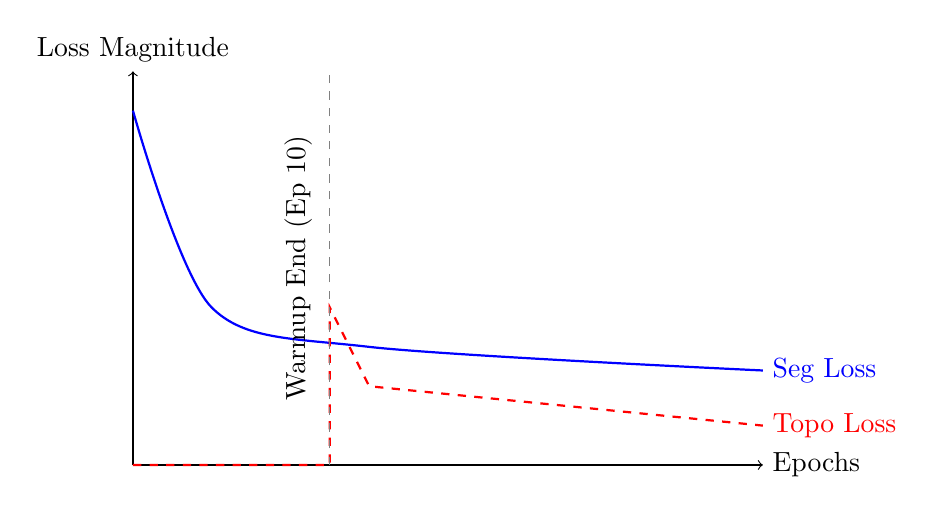
\begin{tikzpicture}
    \draw[->] (0,0) -- (8,0) node[right] {Epochs};
    \draw[->] (0,0) -- (0,5) node[above] {Loss Magnitude};
    \draw[blue, thick] plot [smooth] coordinates {(0,4.5) (1,2.0) (3,1.5) (8,1.2)};
    \node[right, blue] at (8,1.2) {Seg Loss};
    \draw[red, thick, dashed] plot coordinates {(0,0) (2.5,0) (2.5,2.0) (3,1.0) (8,0.5)};
    \node[right, red] at (8,0.5) {Topo Loss};
    \draw[dashed, gray] (2.5,0) -- (2.5,5);
    \node[above, rotate=90] at (2.4, 2.5) {Warmup End (Ep 10)};
    \end{tikzpicture}
    \caption{Schematic of Training Dynamics. I intentionally disabled the Topology Loss for the first 10 epochs (Warmup) to allow the segmentation mask to stabilize.}
    \label{fig:loss_curve}
\end{figure}

\end{document}